
\chapter{The Integrating Decision Support System} % Main chapter title

\label{chapter3} % For referencing the chapter elsewhere, use \ref{Chapter1} 

\lhead{Chapter 3. \emph{The integrating decision support system}} % This is for the header on each page - perhaps a shortened title

The probabilistic decision support techniques for single users we reviewed in Chapter \ref{chapter2} have many advantages: these are coherent from a Bayesian viewpoint and can embed expert judgement when necessary. However the types of demands of current applications, such as the nuclear one we reviewed in Section \ref{sec:nuclear}, require new methods to coherently combine the outputs of networked experts systems in order to provide an integrated study of the whole domain. Therefore, as argued in Chapter \ref{chapter1}, what is needed is an integrating DSS, taking very selected probabilistic outputs from each contributing module and pasting these expert judgements together to provide a comprehensive support. 

We report in this chapter the results of \citet{Smith2015} where we developed a sound statistical methodology to underpin such an integrating system. This provides a framework to faithfully encode all usable and informed expert judgements and data leading to the production of numerical scores ranking the available policies. We envisage that either any of the models we reviewed in Section \ref{sec:prob} or one of the many large
scale hierarchical Bayesian models of temporal spatial processes now in place \citep[e.g.][]{Best2005,Jewell2009, McKinley2014, Wikle2001} informs one of the components of the IDSS. Each of these modules, drawing on experimental and observational evidence supplemented by expert judgement, either directly informs arguments of a decision centre's utility function or provides the necessary input to subsequent components in the process. Different panels of experts in the domain defined by each component oversee and are responsible for the probabilistic outputs of the particular component capturing part of an underlying process. The IDSS is then designed to draw these probabilistic judgements into a single coherent picture to inform policy making. Such a coherent IDSS would thus embody all the qualitative common knowledge and fully defensible domain knowledge of the different panels, and provide baseline judgements around which discussions and modifications could be proposed. 

We describe here how and when it is possible to build such an IDSS and develop statistical methodologies to appropriately guide this knowledge integration. We first introduce a new set of axioms embedding the agreement the group of experts needs to find and, generalising results from \citet{Goldstein96}, we show that these can guarantee the existence of a coherent IDSS. We then define new group Bayesian updating routines for both observational and experimental data for cases where the IDSS is underpinned by a new notion of statistical causality. Lastly, we generalise both current independence conditions and inferential methods for single DMs to groups in a variety of graphical model classes.

The chapter is organised as follows. In Section \ref{sec:features1} we briefly discuss the features of IDSSs and the possible types of support such systems can provide. Section \ref{sec:construction} builds the IDSS methodology and discusses some technical properties that IDSSs need to entertain. In Section \ref{sec:idssexamples} we present some very simple illustrative examples to show the difficulties and the inconsistencies that IDSSs may exhibit.  Section \ref{sec:conditions} presents a number of results that ensure a coherent and faithful IDSS both a priori and after the introduction of observational data. In Section \ref{sec:idsscaus} we then introduce a definition of causality tailored to IDSSs and show that  experimental evidence can be accommodated in these systems whilst retaining coherence. In Section \ref{sec:idssex} we demonstrate that most of the models we reviewed in Sections \ref{sec:nondym} and \ref{sec:dynmod} can be used as integrating overarching structure to aggregate the diverse expert systems' outputs. We conclude with a discussion. 
 
\section{Features of Integrating Systems}
\label{sec:features1}

The description of the RODOS system in Section \ref{sec:nuclear} highlighted the need in current applications for systems capable of drawing different components of the problem together. The IDSS methodology aims at supporting decision centres using expert judgement coming from different panels with different knowledge. We call the \textit{collective} the totality of the experts in the panels, potential users and relevant stakeholders. The IDSS embeds a particular type of \lq{group}\rq ~decision analysis where everyone in the collective accepts to delegate a particular aspect of the problem to the most informed experts  only. The features of this type of decision analysis are summarised in Figure \ref{diagramma}. The collective agrees on the overarching, meaning across panels, probabilistic, preferential and decision structure of the problem the IDSS addresses, as specified by the top three boxes of the diagram in Figure \ref{diagramma}. By overarching statistical model, we mean that the collective identifies the main variables of the problem and the input/output relationships between these, described, for instance, by a set of conditional independence statements or by a graphical model as the network in Figure \ref{networkino}. On the other hand, a preferential overarching model consists of the identification of the attributes of the domain under study together with a set of preferential independences represented, for instance, by a specific utility factorization. In both cases no actual probability and utility elicitations are performed. Then each panel builds its own probabilistic and preferential models, only concerning the domain under its responsibility. These are then integrated into a unique entity to rank policies according to their expected utilities to provide decision support, as indicated by the bottom boxes in Figure \ref{diagramma}.
\begin{figure}
\begin{center}
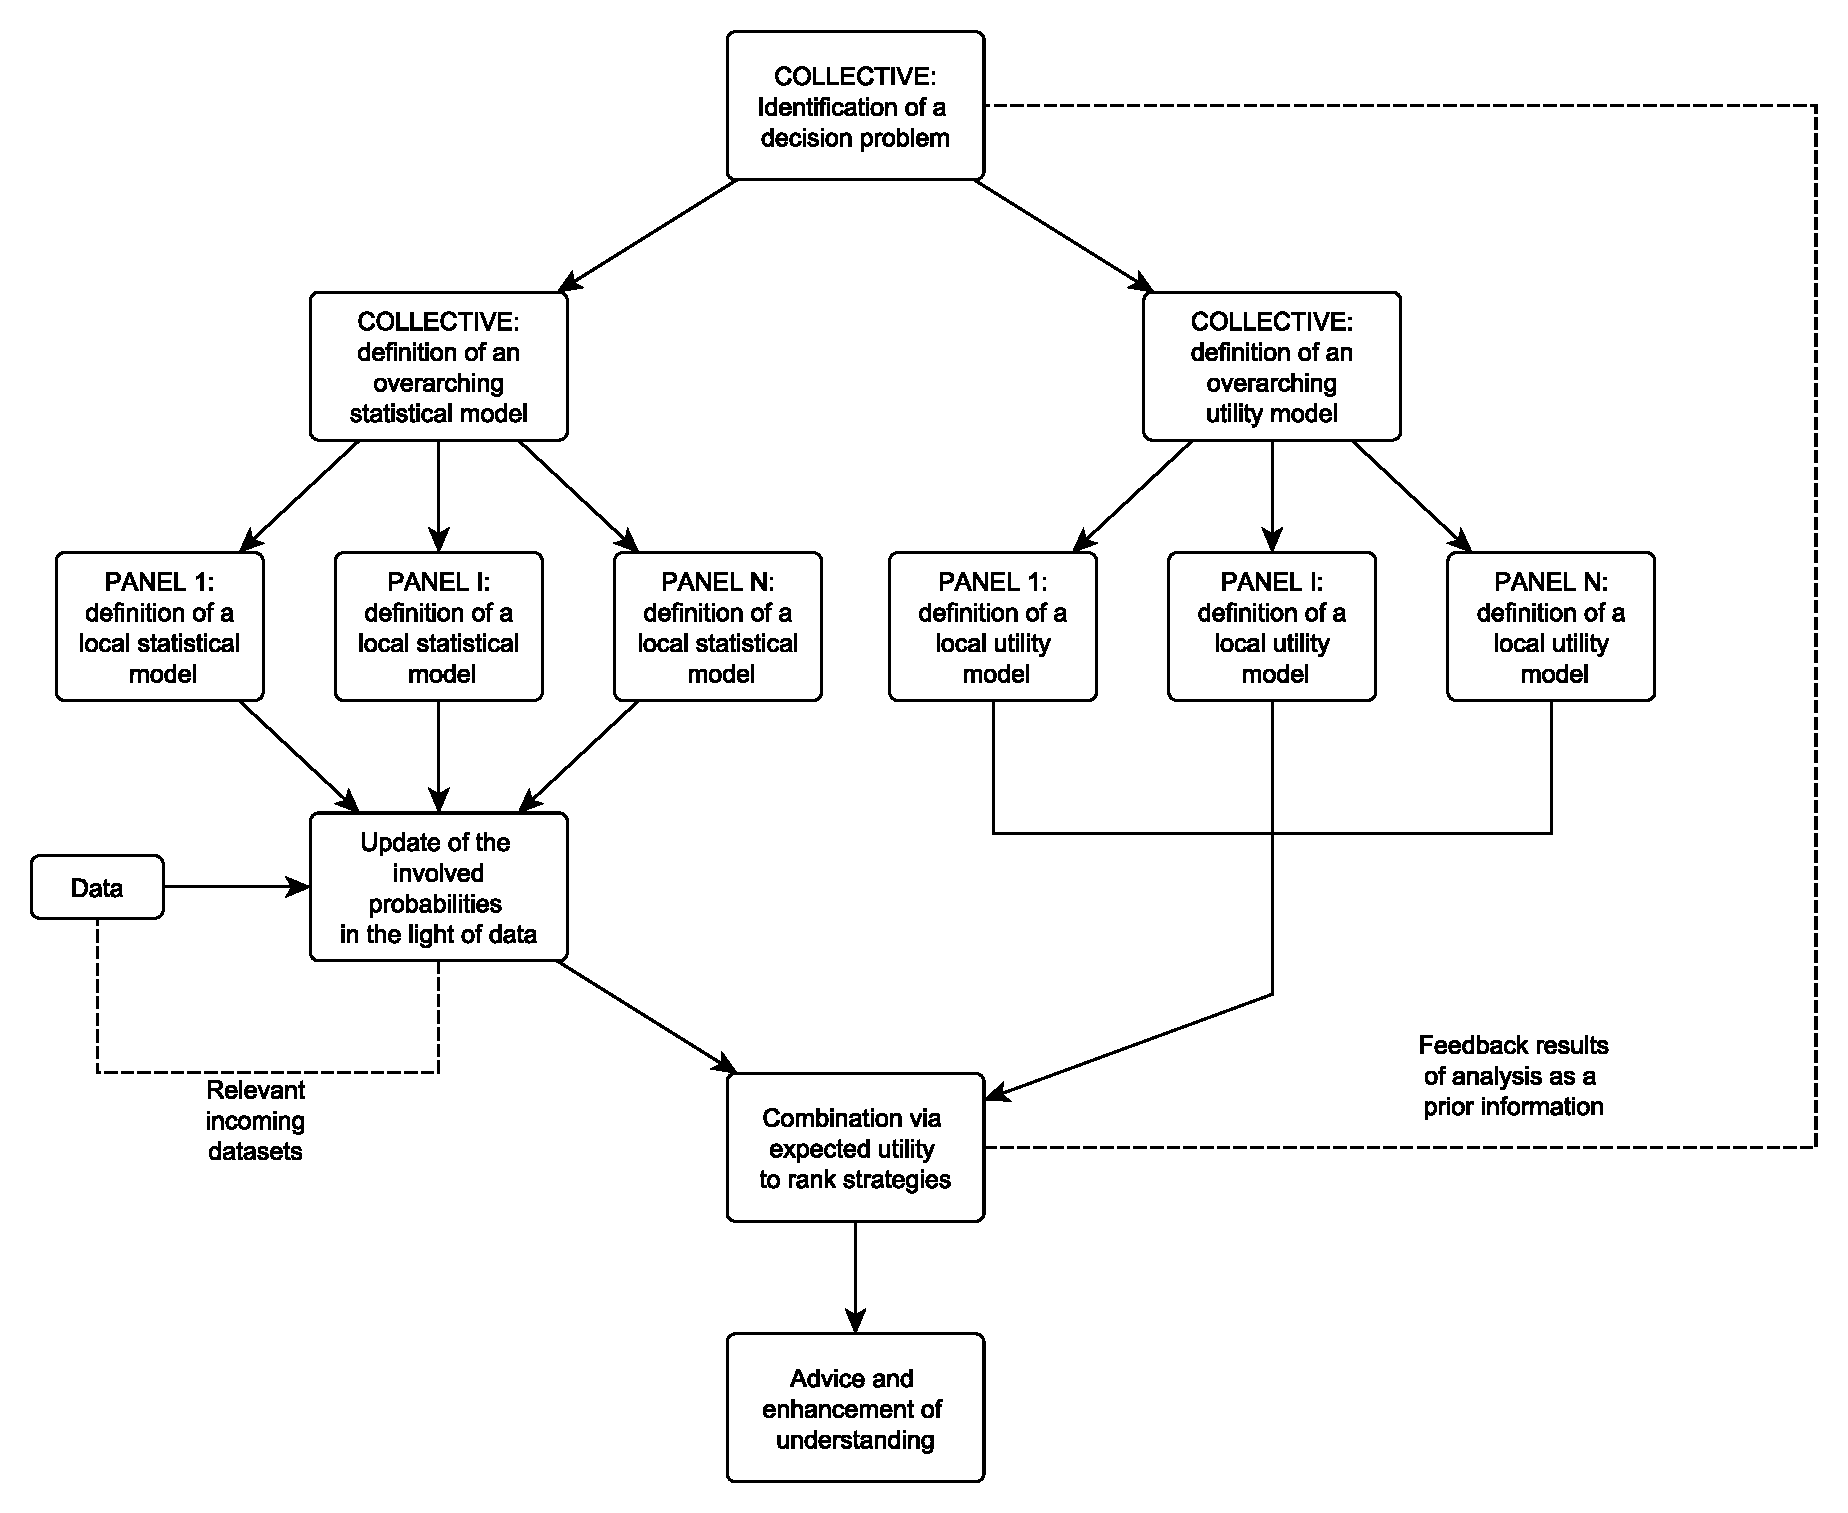
\includegraphics[scale=0.45]{Figure2}
\end{center}
\caption{Structure of a Bayesian decision analysis for a group of distributed experts from \citet{Leonelli2015}, generalising \citet{French97}. \label{diagramma}}
\end{figure}

 One of the challenges to  this process of integration is that no one person or group owns all the relevant probabilistic expert judgements. A first and essential requirement for an IDSS is that its suggestions need to be defensible to the challenges a decision centre might face to the validity of any analysis it might produce. Inputs and outputs of the subsystems and specifically the associated expressions and balancing of uncertainty need not to be self contradictory with each other. Within a Bayesian paradigm this is a \textbf{coherence} requirement over the variables determining the overall expected utility scores, corresponding to the formal separability condition of \citet{Mahoney1996} discussed in Chapter \ref{chapter1}. In a nutshell, this entails that it is possible to define a unique probability distribution over the complete system given the beliefs of the panels. For example if  probability distributions are assigned by two different panels to the amount of contamination to the ground and in water respectively, which have within them an assessment of the air dispersal of contamination, then this assessment has to be the same for the two distributions. If this were not the case, a unique distribution over the IDSS could not be computed and the credibility of the composite would be clearly compromised. 

A second requirement for a practical IDSS is that the panels deliver \textit{sufficiently rich} sets of information, so that they together provide enough information to compute the expected utility function. This is in general impossible unless some assumptions are made by the collective. Note that some parts of the process under examination may be very well studied and modelled, but the knowledge about others is often patchy. So for instance, dispersal models are now well established and able to compute a variety of summaries  of the spread of contamination, whilst the estimates of the political effects of the accident on the stability of the affected regions often come only in the form of expert judgement.  

A third important property increasing the defensibility of the outputs of an IDSS is that this incorporates the \textit{fullest} and \textit{most reliable} possible \textit{evidence} within its probability specifications. This in turn requires that expert judgements are provided only by the most informed panels. However, IDSSs that are coherent a priori might not be so any more after the introduction of data. For this reason, filters checking the data that is admitted in the IDSS to perform Bayesian updating need to be implemented. If these filters are in place, then panels can produce revised estimates of the required quantities for the decision analysis, improving the overall suggestions the system is producing and consequently supporting more focused decision making. 


It is also often necessary for the IDSS to be used in real time, during the unfolding of a certain crisis. Modules are now designed so that they are fast. However this is not sufficient to guarantee that the composite as a whole is able to run quickly and still retain its coherence. To achieve this, a necessary property is that the system is \textbf{distributed} (or \textit{modular}). By this we mean that the composite system calculates all functions needed to evaluate the expected utility associated with its available decisions from outputs delivered by individual panels, where these are allowed to be functions of other panels' outputs. There are several advantages that derive from structuring a problems so that the ensuing support is distributed:
\begin{enumerate}
\item first, because the responsibility for each aspect of the analysis can be devolved to \textit{appropriate} panels of experts, these are then more likely to deliver better calibrated judgements.  This in some ways guarantees the semantic separability of \citet{Mahoney1996}. The whole system might therefore be expected to be more robust to the misspecification of beliefs \citep{Cooke1991a}. On the other hand, if the system needs to be changed in the light of unexpected developments or unplanned consequences, under suitable conditions, the management of these new developments need only be addressed \textit{autonomously} by the relevant panels. These simply adapt their individual forecasts and inputs in the light of the new scenario they face. These adjustments can then be folded back into the system to provide  a revised output of the relevant modules for other panels to use for their inputs;
\item second, the output of a distributed IDSS can produce answers to queries by decision centres about the premises on which it is based and the calculations of its outputs, by directing the query to the relevant panels. A route along which the relevant panels can be queried as to the reasons of their contribution to the expected utility scores is described in Figure \ref{possuse}, which shows the different levels of support that can be implemented into an IDSS. When queried, generic DSSs are usually able to present justifications for the overall expected utility scores and the ranking of the available policies (third box of the second column from the left of Figure \ref{possuse}). However IDSSs are able to provide an additional level of support. The system's distributivity permits the IDSS to justify its suggestions in terms of the modules outputs, since expected utilities are functions of these (see the bottom box of the second column from the left of Figure \ref{possuse}). If these systems did not exhibit this distributivity property, then such devolution may not be possible and so any support would be much less transparent. This feature increases both the comprehensibility and the feasibility of testing that, as argued by \citet{Mahoney1996}, current DSSs need to address;
\item third, distributivity ensures that different decision centres can be given the option of choosing different modules to model the various components of the problem. For example, in nuclear emergency management, different countries often prefer to predict the spread of the contamination using  their national agencies' diffusion models;
\item lastly, although many of the modules are probabilistic, distributivity allows us not to construct a single composite probabilistic model: such a universal system would be infeasibly large and no one would own the joint distributions of the unwieldy number of random variables. Even if it were possible to build such a system, the component modules are usually being constantly revised both in their structure and inputs. Were such an overarching probabilistic system possible to build, it would therefore be obsolete before it was completed.  
\end{enumerate}

\begin{figure}
\begin{center}
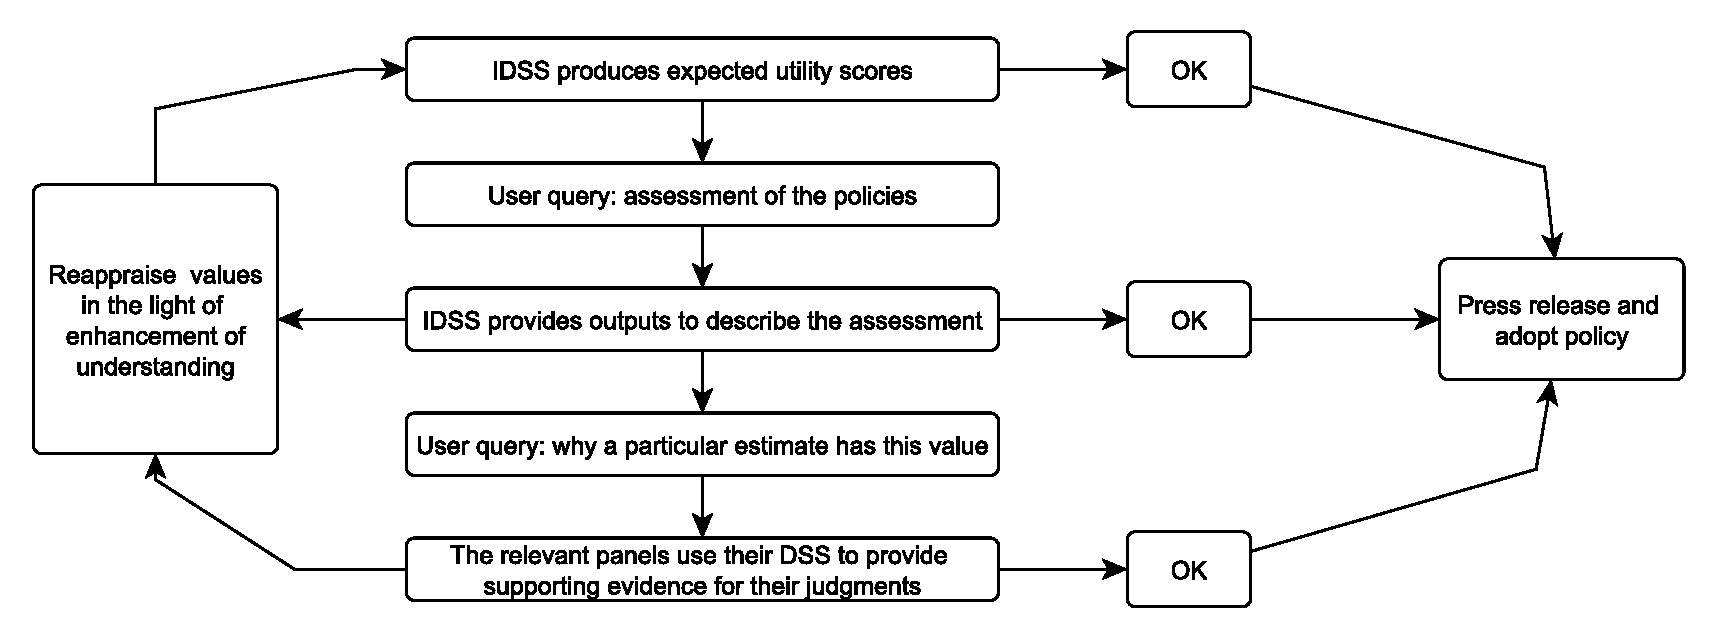
\includegraphics[scale=0.5]{Figure1}
\caption{Description of the possible use of an integrating decision support system for a decision analysis. \label{possuse}}
\end{center}
\end{figure}


\section{Construction of Integrating Systems}
\label{sec:construction}
\subsection{Some Technical Structure}
A domain is defined by a large number of random variables $\bm{Y}=(Y_i)_{i\in[n]}^{\T}$. As often in practice, the problem is heterogeneous and therefore assume different components of the problem, denoted as $\bm{Y}_i$, are evaluated and overseen by $m$ different panels $\{G_i: i\in[m]\}$ of domain experts, $[m]=\{1,\dots, m\}$. The implicit, albeit virtual, owner of these beliefs is henceforth referred to as the SB. Let $\bm{\mathcal{D}}$ be a decision space including the available policies $\bm{d}\in\bm{\mathcal{D}}$.  The SB needs to process the necessary probabilistic features delivered by the different panels to calculate various statistics of a potential decision centre's reward vector $\bm{R}$, some function of both $\bm{Y}$ and $\bm{d}$. 

Panel $G_i$ donates to the SB various summaries of the distribution of the subvector $\bm{Y}_i\;|\;\bm{d}$ under its jurisdiction, conditional on certain measurable functions $\{L_i(\bm{Y}_i):L_i\in\mathcal{L}_i\}$, where $\mathcal{L}_i$ could be empty, $i\in[m]$. For instance, in a generic graphical model the set $\mathcal{L}_i$ might consist of the possible configurations of values of the parents of $\bm{Y}_i$. Assume that panel $G_i$, $i\in [m]$, is able to make available the following:
\begin{enumerate}
\item a collection of summary statements about the measurements under its jurisdiction
\begin{equation*}
\Psi_i^{\bm{y}|\bm{\theta}}=\{\Psi_i^{\bm{y}|\bm{\theta}}(\bm{\theta}_i,L_i,\bm{d}): \bm{\theta}_i\in\bm{\Theta}_i,\;L_i\in\mathcal{L}_i,\;\bm{d}\in\bm{\mathcal{D}}\}.
\end{equation*}
These inform the IDSS about the likelihoods
$f_i(\bm{y}_{i}\;|\;\bm{\theta }_{i},L_i, \bm{d})$, $L_i\in \mathcal{L}_i$, $\bm{d}\in \bm{\mathcal{D}}$, where $\bm{\theta }_{i}\in \bm{\Theta} _{i}$ parametrise the (possibly conditional) density of $\bm{Y}_i\;|\;\bm{\theta},\bm{d}$. For example, if $\bm{Y}$ were discrete and finite, then each panel might be asked to provide certain contingency tables over $\bm{Y}_{i}\;|\;\bm{\theta},\bm{d}$, conditional on each $L_{i}\in \mathcal{L}_{i}$. In this case $\bm{\theta}_{i}\in \bm{\Theta} _{i}$ would be the probabilities within all these tables. An important note to make here is that there is often a typically much longer vector of parameters $\bm{\phi}_{i}\in \bm{\Phi} _{i}$ over which $G_{i}$ has beliefs but which are not directly relevant to the distribution of the predictions the IDSS needs to deliver;
\item a set of summaries about its prior beliefs  
\begin{equation*}
\Psi _{i}^{\bm{\theta} }=\left\{ \Psi _{i}^{\bm{\theta} }(L_i,\bm{d}): L_i\in\mathcal{L}_i,\;\bm{d}\in\bm{\mathcal{D}} \right\}, 
\end{equation*}
from the panel prior densities $\pi_i(\bm{\theta}_i\;|\;L_i,\;\bm{d})$, $\bm{d}\in\bm{\mathcal{D}}$, $L_i\in\mathcal{L}_i$. In the above example this would be a joint probability distribution over the entries of the relevant contingency tables. Note that often these panel beliefs are calculated by marginalising out $ \bm{\phi }_{i}\in \bm{\Phi}_{i}$;
\item from these two sets of quantities, the calculated collection of summaries 
\[
\Psi _{i}^{\bm{y}}= \left\{ \Psi _{i}^{\bm{y}}(L_i,\bm{d}):L_i\in\mathcal{L}_i,\; \bm{d}\in \bm{\mathcal{D}}\right\} ,
\]
about the marginal distribution of $\bm{Y}_{i}\;|\;\bm{d}$ conditional on each event $L_{i}$. Here $\Psi _{i}^{\bm{y}}(L_{i},\bm{d})$ is calculated from $\Psi_{i}^{\bm{y}|\bm{\theta }}(\bm{\theta }_{i},L_{i},\bm{d})$ by $G_{i}$ marginalising over $\bm{\theta }_{i}$ using $\Psi _{i}^{\bm{\theta}}(L_{i},\bm{d})$ for each $L_{i}\in \mathcal{L}_{i}$, $\bm{d}\in \bm{\mathcal{D}}$. In the example above, these might be the corresponding expected conditional tables where expectations are taken across the probability vectors $\bm{\theta }_{i}$.  These are the quantities the IDSS uses to calculate its expected utility scores associated with its available decisions and to help a decision centre to determine its most efficacious policy.
\end{enumerate}

\subsection{Common Knowledge Axioms}
Suppose that after a series of decision conferences (see Section \ref{sec:decconf}) held jointly across the panels, stakeholders and potential users, all have agreed the types of decisions the IDSS  supports to a sufficient level of specificity to provide an agreed qualitative framework across all interested parties around which a quantitative structure can be built. To this purpose we make three assumptions.

\begin{axiom}[policy consensus]
\label{axiom:policy}
The collective agrees the class of decision rules $\bm{d}\in \bm{\mathcal{D}}$ examined by the IDSS.
\end{axiom}

This class of feasible policies considered  depends not only on what is logical, such as when various pieces of information are likely to become available, but also what might be allowable, either legally or for other reasons.

\begin{axiom}[utility consensus]
\label{axiom:utility}
The collective agrees on the class $\mathcal{U}$ of utility functions supported by the IDSS.
\end{axiom}
In the complex multivariate settings we address here, the utility function $u(\bm{r},\bm{d})$ needs to entertain certain types of preferential independence in order to allow for a distributed analysis. In this chapter we assume that some additive or multilinear factorisation is believed to hold. In Chapter \ref{chapter4} we introduce a large class of partial utility independence models, of which additive and multilinear factorisations can be seen as a special case, that can allow for distributed analyses. Again the choice of $\mathcal{U}$ is often resolved using decision conferencing across the members of the collective.

\begin{axiom}[structural consensus]
\label{axiom:structural}
The collective agrees the variables $\bm{Y}$ defining the process - where for each $\bm{d}\in \bm{\mathcal{D}}$, each $u\in \mathcal{U}$ is a function of $\bm{Y}$ - together with a set of qualitative statements about the dependence between various functions of $\bm{Y}$, $\bm{\theta }$ and $\bm{d}$. Call this set of assumptions the \textbf{structural consensus set} and denote this by $\mathcal{J}$.
\end{axiom}
This last consensus might be expressible through agreement that a particular graphical or conditional independence structure across not only the distribution of $ \bm{Y}\;|\;\bm{\theta }, \bm{d}$,  but also over the one of $\bm{\theta }\;|\;\bm{d}$ is valid, $\bm{d}\in\bm{\mathcal{D}}$. For instance, the structural consensus might include the assumption of local and global independence of the parameter vector in a BN model (see Section \ref{sec:BN}). Other information that might be included in $\mathcal{J}$ could be a consensus about certain structural zeros or known logical constraints (such as probabilities needing to add to one and be non-negative).

\begin{definition}
Call the set of assumptions forming the union of the utility, policy and structural consensus $\left( \mathcal{U},\bm{\mathcal{D}},\mathcal{J}\right) $ the \textbf{Common Knowledge-class (CK-class))}.
\end{definition}

Technically, we can think of the CK-class as the \emph{qualitative} beliefs that are shared as common knowledge by all  panel members and potential users. The CK-class represents the foundation around which all inference within the IDSS takes place. Note that this depends not only on the domain and needs of users of the system, but also on the constitution and knowledge bases of the panels.

We now provide a list of the types of quantitative information needed to populate the CK-class and to calculate the expected utility $\bar{u}(\bm{d})$ of the available decisions $\bm{d}\in\bm{\mathcal{D}}$. To achieve this, the SB  needs the decision centre's choice of $u(\bm{r},\bm{d})\in \mathcal{U}$ together with enough probabilistic information to calculate the expectations of these utilities. At worst this might need to be the full distribution of $\bm{R}$. Alternatively and more commonly for typical choices of $\mathcal{U}$, all that might be needed is the distribution of the margins on certain specific functions of $\bm{R}$ or simply some summaries. 

\begin{axiom}[quantitative delegation consensus]
\label{axiom:quantitative}
The collective agrees to take on the sample summaries $\Psi _{i}^{\bm{y}|\bm{\theta} }$, the panel prior beliefs $\Psi _{i}^{\bm{\theta} }$ and the panel marginal inputs $\Psi _{i}^{\bm{y}}$ delivered by $G_{i}$ as its own, $i\in[m]$.
\end{axiom}
This axiom essentially demands that everyone agrees that it is appropriate to defer their judgements to the panel which is most informed about each domain vector. A sufficient set of qualitative conditions justifying its use is given in Section \ref{sec:coherence}.
\subsection{Properties of Integrating Systems}
The above axioms specify the structure of the IDSS, but these do not in general guarantee that the output of the system provides coherent decision support. In this section we introduce concepts that characterise what a \lq{good}' IDSS is.
\begin{definition}
\label{def:adequacy}
An IDSS is \textbf{adequate} for a CK-class if the SB can unambiguously calculate the expected utility scores, for any decision $\bm{d}\in \bm{\mathcal{D}}$ and any utility function $u\in \mathcal{U}$, from the panel marginal inputs $\Psi _{i}^{\bm{y}}$ delivered by $G_{i}$, $i\in[m]$.
\end{definition}
One particular useful refinement of adequacy is the following.
\begin{definition}
An IDSS is \textbf{universally adequate} for a CK-class if the SB can unambiguously calculate the distribution of $\bm{R}$ from the panel marginal inputs $\Psi _{i}^{\bm{y}}$ delivered by $G_{i}$, $i\in[m]$.
\end{definition}
An adequate IDSS is able to derive a unique score for each option on the basis of the individual panels' inputs. An IDSS clearly cannot be fully functional unless it has this property. For a universally adequate IDSS this is true regardless of the form of $\mathcal{U}$.

To be defensible the IDSS needs another property.
\begin{definition}
An IDSS is \textbf{sound} for a CK-class if it is adequate and the SB can coherently admit all the assessments $\Psi_{i}^{\bm{y}|\bm{\theta} },\Psi _{i}^{\bm{\theta }}$ and $\Psi _{i}^{\bm{y}}$, $i\in[m]$, as her own, the SB's underlying belief model being shared with those of the relevant panels.
\end{definition}
A sound IDSS does not necessarily need to embody the \emph{genuine} beliefs held by the panel members and potential users based on the totality of their own personal evidence. This would be too much to ask since much of this evidence might be from poorly designed experiments, formally unjustifiable to the public or simply anecdotal. However the sound IDSS does present a defensible and conservative position all panellist should be happy to communicate, and provide a benchmark for further discussion. Most importantly soundness guarantees that the beliefs are formally separable.

A property we  always assume to be part of a CK-class is that panels are variationally independent, i.e $\bm{\Theta}=\bigtimes_{i\in[m]}\bm{\Theta}_i$ (see Definition \ref{def:varind}). If this were not the case, then beliefs of one panel would be necessarily shared with the ones of other panels. In such case both soundness and distributivity could not hold for IDSSs.

\section{Illustrative Examples}
In this section we present a series of simple and intuitive examples illustrating the IDSS machinery and the dangers associated to non coherent belief specifications. 

\label{sec:idssexamples}
\subsection{Strong Adequacy and Soundness a Priori.}
Let $m=2$, $\bm{R}=\bm{Y}=(Y_1,Y_2)^\T$, where $Y_i$ is binary, $i\in[2]$, $\bm{\theta}$ parametrise the density of $(Y_1,Y_2)\;|\;\bm{\theta},\bm{d}$, and suppose a generic decision space $\bm{\mathcal{D}}$.  Here the random variable $Y_1$ is an indicator of whether or not the contamination is dispersed in the area and $Y_2$ is an indicator of whether or not the population is affected by the accident. The sample summary delivered by $G_1$  is $\theta_1=\mathbb{P}(Y_1=1\;|\;\theta_1,\bm{d})$, whilst $G_2$ delivers $\{\theta_{20},\theta_{21}\}$, where $\theta_{20}=\mathbb{P}(Y_2=1\;|\;Y_1=0,\theta_{20},\bm{d})$ and $\theta_{21}=\mathbb{P}(Y_2=1\;|\;Y_1=1,\theta_{21},\bm{d})$.   Write $\bm{\theta}_2=(\theta_{20},\theta_{21})^\T$. Note that in this case $\mathcal{L}_1$ is empty, whilst $\mathcal{L}_2$ consists of the possible outcomes of $Y_1$.

  If a CK-class includes $\mathcal{U}$, an arbitrary utility on $\bm{R}$, then, since the above probabilities fully define the model, for strong adequacy the SB needs to be able to calculate the expected joint probability table of $\bm{Y}\;|\;\bm{d}$. Specifically this corresponds to the expected values $\bar{\bm{\mu }}=( \bar{\mu }_{00},\bar{\mu }_{01},\bar{\mu }_{10},\bar{\mu }_{11})^\T $ of $\bar{\bm{\theta }}=( \bar{\theta }_{00},\bar{\theta }_{01},\bar{\theta }_{10},\bar{\theta }_{11})^\T $, where by definition 
\begin{equation*}
\begin{array}{cccc}
\bar{\theta }_{00}=(1-\theta _{1})(1-\theta _{20}), & \bar{\theta }_{01}=(1-\theta _{1})\theta _{20},&
 \bar{\theta }_{10}=\theta_{1}(1-\theta_{21}), & \bar{\theta }_{11}=\theta _{1}\theta _{21}.
\end{array}
\label{binaryexdep}
\end{equation*}
Suppose that the qualitative statement $\theta_1\independent \bm{\theta}_2\;|\;\bm{d}$ is in the  CK-class for every $\bm{d}\in\bm{\mathcal{D}}$. Letting $\mu_1=\E(\theta_1\;|\;\bm{d})$ and $\bm{\mu}_2=(\mu_{20},\mu_{21})^\T=\left(\E(\theta_{20}\;|\;\bm{d}),\E(\theta_{21}\;|\;\bm{d})\right)^\T$,  we then have that 
\begin{equation*}
\begin{array}{cccc}
\bar{\mu}_{00}=(1-\mu_{1})(1-\mu_{20}), & \bar{\mu }_{01}=(1-\mu _{1})\mu _{20},&
 \bar{\mu }_{10}=\mu_{1}(1-\mu_{21}), & \bar{\mu }_{11}=\mu _{1}\mu_{21}.
\end{array}
\label{exp uti}
\end{equation*}%
Suppose $G_{1}$ and $ G_2$ make available their expectations  $\mu _{1}$ and $ \bm{\mu }_{2}$,  respectively.
Then, because of the independence statements between the parameter vectors in the structural consensus, the IDSS is a strongly adequate system with the delivered assessments, 
providing the SB with all the information needed to calculate the expected utility functions using the formulae in (\ref{exp uti}). It is also sound since these inputs are consistent with any probability model over $(\bm{Y},\theta _{1},\bm{\theta }_{2})\;|\;\bm{d}$ with these expectations and the independence between the parameter vectors.

It is not a trivial condition that SB's beliefs required for either adequacy or strong adequacy are a function of the panels beliefs only. For example the full joint distribution of $\bm{Y}\;|\;\bm{\theta},\bm{d}$ is not fully recoverable from the marginal densities over $\theta_1\;|\;\bm{d}$ and $\bm{\theta}_2\;|\;\bm{d}$ two different panels might simply provide, since the SB cannot derive the conditional covariance between $\theta_{1}$ and $\bm{\theta }_{2}$ given $\bm{d}$ which was needed to calculate the conditional covariance between $Y_{1}$ and $Y_{2}$ given $\bm{d}$.

\subsection{Adequacy and the Risk of non Soundness.}
\label{sec:adequacy}
Assume a CK-class gives $\bm{Y} $ the same meaning as in the previous  section. However add to the CK-class the additional structural assumption that $Y_{2}\independent Y_{1}\;|\;\theta_{1},\bm{\theta} _{2},\bm{d}$ whatever decision $\bm{d}\in \bm{\mathcal{D}}$ is made. Thus, once the probabilities of these events are known, it is generally accepted that learning that contamination has been introduced in the environment does not affect the judgements about the health effects on the population. Note that in this case $\mathcal{L}_i$ is empty, $i\in[2]$.  Suppose $G_{1}$ delivers the beta distributions $\Be(p_{1},q_{1})$ for $\theta _{1}=\mathbb{P}(Y_{1}=1\;|\;\theta_1,\bm{d})$ and  $G_{2}$ has the  beta distributions $\Be(p_{2},q_{2})$ for $\theta _{2}=\mathbb{P}(Y_{2}=1\;|\;\theta_2, \bm{d})$. Note that because of the structural assumption above, our notation is now such that $\theta_{2}=\theta _{20}=\theta _{21}$. Consider two possible CK-classes where a decision centre is known to draw its utilities $u_{i}\in \mathcal{U}_{i}$, $i\in[2]$, from one of the families below 
\begin{align*}
u_{1}(y_{1},y_{2},\bm{d}) &=a_1+b_{11}y_{1}+b_{12}y_{2}, \\
u_{2}(y_{1},y_{2},\bm{d}) &=a_2+b_{2}y_1y_2,
\end{align*}
where $a_1,a_2\in\mathbb{R}$ and $b_{11},b_{12},b_{2}\in\mathbb{R}_{>0}$. If $\mathcal{U}_{1}$ is in the CK-class then the SB needs only $G_{i}$ to supply its prior mean $\mu _{i}$ of $\theta _{i}\;|\;\bm{d}$, $i\in[2]$, where $\mu_i=p_i(p_i+q_i)^{-1}$, in order to calculate the expected utility associated to $\bm{d}$.  So there is some redundancy in the delivery of $G_{1}$ and $G_{2}$: panels only need to specify their prior means for every $\bm{d}\in \bm{\mathcal{D}}$ and not their whole marginal distributions over $\theta _{1}\;|\;\bm{d}$ and $\theta _{2}\;|\;\bm{d}$.

However, if $\mathcal{U}_{2}$ is in the CK-class, then the SB needs to be able to calculate 
\[
\mathbb{E}(Y_1Y_2\;|\;\theta_1,\theta_2,\bm{d})=\mathbb{E}\left( \theta_{1}\theta _{2}\;|\;\bm{d}\right),
\] 
and the panels prior means are no longer necessarily  adequate. For this to be so the CK-class then needs the additional assumption $\theta _{1}\independent \theta _{2}\;|\;\bm{d}$. In this case 
\[
\mathbb{E}(Y_1Y_2\;|\;\theta_1,\theta_2,\bm{d})=\mathbb{E}(\theta_1\theta_2\;|\;\bm{d})=\mu _{1}\mu _{2},
\]
 and the IDSS retrieves adequacy. However, this additional common knowledge statement needs to be credible. For instance, suppose that $p_{1}+q_{1}=p_{2}+q_{2}= \sigma$, so that $\Theta _{1}\times \Theta _{2}$ is parametrised by $\left( \mu_{1},\mu _{2},\sigma \right) $. Then, it is easily checked that the collective can specify its joint beliefs over the probabilities on the 4 events of the form $\left( y_{1},y_{2}\right)$, $y_{1},y_{2}=[1]^0=[1]\cup\{0\}$, with a Dirichlet distribution, $\Di(a_{00},a_{10},a_{01},a_{11})$, where
\[
\begin{array}{cccc}
p_{1} =a_{10}+a_{11}, &
q_{1} =a_{00}+a_{01}, &
p_{2} =a_{01}+a_{11}, &
q_{2} =a_{00}+a_{10},
\end{array}
\]
since, from well known properties of the Dirichlet distribution \citep[see e.g.][]{Geiger1997}, this is consistent with the given margins. However this collective prior is \emph{not} consistent with the independence assumption $\theta_1\independent \theta_2\;|\;\bm{d}$ given above. From the properties of the Dirichlet (see Appendix \ref{sec:multidir}), the SB's mean of $\theta_1\theta_2\;|\;\bm{d}$ is given by $a _{11}\sigma^{-1}$ where $\sigma =a _{00}+a_{10}+a_{10}+a_{11}$, which is not equal to $\mu _{1}\mu _{2}$ unless $\rho = \sigma^{-2}\left( a_{11}a_{00}-a_{10}a_{11}\right)=0$, since $\rho$ is the unique solution to 
\begin{equation*}
\mu_1\mu_2=a_{11}\sigma^{-1}\Longleftrightarrow \frac{(a_{10}+a_{11})(a_{01}+a_{11})}{\sigma^2}=\frac{a_{11}}{\sigma}.
\end{equation*} 
So the SB cannot calculate $\E(\theta_1\theta_2\;|\;\bm{d})$ from the inputs delivered by the panels. In fact $\E(\theta_1\theta_2\;|\;\bm{d})=\mu _{1}\mu _{2}+\rho $, which is  unidentified from the margins provided by the panels. 

\subsection{Bayesian Updating}
Ideally we would like the IDSS to be distributed so that panels can autonomously update their probabilistic beliefs as they receive new information. To illustrate how distributivity might be possible, suppose a random vector $\left( \bm{X}_{1},\bm{X}_{2}\right) $ is sampled from the same population as $\left( Y_{1},Y_{2}\right) $ in the model above and that, for each $\bm{d}\in \bm{\mathcal{D}}$, $\theta _{1}\independent \theta_{2}\;|\;\bm{d}$  is in the CK-class. Each panel $G_{i}$ next refines its probabilistic assessments by observing its own separate randomly sampled populations, $\bm{x}_{i}$, and then updates its beliefs, given each $\bm{d}\in \bm{\mathcal{D}}$, from $\pi _{i}(\theta _{i}\;|\;\bm{d})$ to $\pi_{i}(\theta _{i}\;|\;\bm{d},\bm{x}_{i})$, $i\in[2]$.

Now the two panels need to deliver only their respective posterior means $\E(\theta_i\;|\;\bm{d},\bm{x}_i)$, $i\in[2]$, $\bm{d}\in \bm{\mathcal{D}}$. The SB can then act coherently and as if she had processed this information on her own: the IDSS is therefore sound and distributed. So in particular once all the data accommodated into the composite is of the form of autonomous random sampling, inference can be simply delegated to the appropriate panels who simply periodically and independently revise their judgements.

However note that parameter independence is critical for this distributivity property. Assume the SB uses the additive utility class $\mathcal{U}_{1}$, but that there are no clear reasons why $\theta _{1}\independent\theta _{2}\;|\;\bm{d}$ should be in the CK-class, so that the prior over $\theta _{2}$  needs to be a function of $\theta _{1}$ for at least some $\bm{d}\in \bm{\mathcal{D}}$. Then with these beliefs, were the SB a single agent, she would for example draw on what she learns about $\theta _{1}$ from  $\bm{x}_{1}$  to update her beliefs about $\theta _{2}$. So her posterior density on $\theta _{2}\;|\;\bm{d}$ 
\begin{equation*}
\pi _{2}(\theta _{2}\;|\;\bm{x}_{1},\bm{x}_{2},\bm{d})=\int_{0}^{1}\pi _{2}(\theta _{2}\;|\;\theta_{1},\bm{x}_2,\bm{d})\pi_1(\theta _{1}\;|\;\bm{x}_1,\bm{d})\dr\theta _{1},
\end{equation*}%
has associated expectation $\E(\theta_2\;|\; \bm{x}_1,\bm{x}_2,\bm{d})\neq \E(\theta_2\;|\;\bm{x}_2,\bm{d})$ in general. Therefore the SB using $\E(\theta_i\;|\;\bm{x}_i,\bm{d})$,  $i\in[2]$, will \emph{not} be acting as a single Bayesian would. So the system is no longer sound. Although when supporting evidence remains unseen the SB appears to act coherently, her analyses are indefensible if subsequently challenged. 

\subsection{Learning with Randomised Samples.}
\label{sec:nonrandomized}
Note that even if the parameter independence $\theta_1\independent \theta_2\;|\;\bm{d}$ is justified a priori, the assumption that data collected by the two panels and individually used to adjust their beliefs does not inform both parameters is also a critical one. Continuing the example above  and assuming $u\in \mathcal{U}_{2}$, suppose that $G_{1}$ and $G_{2}$ both see the results of the experiment in Table \ref{table:example}, where $100$ units from the population are randomly sampled, for a particular $\bm{d} \in \bm{\mathcal{D}}$. Each panel uses this experiment to update its respective marginal distributions over $\theta _{i}\;|\;\bm{d}$, $i\in[2]$.

\begin{table}
\begin{center}
\begin{tabular}{ccccc} 
$Y_1/Y_2$&0&1&&\\
0&5&45&50&$n-x_1$\\
1&45&5&50 &$x_1$\\
&50&50&100&\\
&$n-x_2$&$x_2$&&
\end{tabular}
\end{center}
\caption{A random sampled experiment for the example in Section \ref{sec:nonrandomized}. \label{table:example}}
\end{table}

Then, if both began with a prior symmetric about $0.5$, each would believe that its posterior mean would still be equal to one half. So were $\theta _{1}\independent \theta _{2}\;|\;\bm{d}$ in the CK-class and assuming that all evidence the individual panels use is from the marginal counts only, the IDSS would assign $\E(\theta_1\theta_2\;|\;x_1,x_2,\bm{d})=0.25$. In contrast, were the  SB to see this table, assuming $\theta _{1}\independent \theta _{2}\;|\;\bm{d}$ a priori with fairly uninformative priors on the two margins, then her posterior mean of $ \theta_1\theta_2\;|\;\bm{d}$ would be approximately $0.05$, which is way different than the estimate above. No one may have access to the joint table but just its marginal counts. So unless a protocol is adopted by the IDSS preventing data inducing this type of ambiguity into the distributed IDSS,  then this system might be grossly misleading. Interestingly if the CK-class does not include $Y_{2}\independent Y_{1}\;|\;\theta _{1},\theta_{2}$, then we can prove below that in the extended system there is a simple solution to this problem. This is because the given sample data appears to challenge the assumption $Y_{2}\independent Y_{1}\;|\;\theta _{1},\theta _{2},\bm{d}$. When an observed likelihood destroys the prior independence of the parameters in the two posterior margins, the useful distributive property is lost because  the independence between $\theta_{1}$ and $\theta_{2}$ given $\bm{d}$ no longer holds a posteriori. 

So we have illustrated above that even in the simplest of networks, considerable care needs to be exercised before an IDSS can be expected to work reliably. In the next section we prove some conditions which ensure an IDSS is sound both a priori and a posteriori.

\section{Conditions for a Coherent Integrating System}
\label{sec:conditions}

Having illustrated above some of the challenges faced by an IDSS, in this section we investigate sufficient conditions leading to coherence and distributivity. We are able to demonstrate that if  panels are constructed wisely and that care is taken in defining what observational data is allowed to inform IDSSs, the necessary conditions are not overly restrictive.

However, an IDSS needs to have an appropriate protocol which systematically excludes or delays some pieces of information. Suppose a sequence of datasets is presented to the IDSS as time progresses. We call the information that such a  protocol allows into the system up to time $t$ the \emph{admissible evidence} and denote it by $I_{+}$. This mirrors the information set in the definition of the DLM model class of Section \ref{sec:DLM}. The types of information excluded or delayed by this protocol are simply those that either cause ambiguity or lack of consensus and therefore break the distributivity of the IDSS. In this sense the beliefs of the IDSS are conservative. Of course all statements in an IDSS simply provide a benchmark from which further discussion - possibly involving  more contentious sources of evidence - can ensue before acts are decided. But we argue that primarily an IDSS needs to be able to deliver outputs based on considered and agreed inputs from the expert panellist and that its judgements  have a supporting narrative associated with them, which can be appraised and, if necessary, replaced during any given crisis as described in Figure \ref{possuse}.

Of course, that there exist relevant protocols for the selection of good quality evidence for decision support is often assumed even for single agent systems, but its explicit statement is frequently omitted. For instance, the Cochrane reviews are considered to be the gold standard in decision support for medical treatments  \citep{Higgins2008}. Their purpose is to pare away information which might be ambiguous and potentially distort inferences through a highly-developed and trusted set of principles relevant to the domain.  Here, we assume that panels can select suitable evidence, mirroring Cochrane in ways relevant to their domain. We also assume that such relevant analysis can be performed locally. We demonstrate below that conditions justifying this strongly relate to certain conditional independence statements leading  to the separability across different panel parameters of the observed likelihood of portfolios of data.


\subsection{Group Conditional Independences}
To deduce these independences,  let $I_{CK}^{t}\subseteq I^t_{+}$ denote all the admissible evidence which is common knowledge to all panel members at time $t$ and $I_{ij}^{t}$ denote the subset of $I^t_+$ panel $G_i$ would use at time $t$ if acting autonomously to assess its beliefs about $\bm{\theta }_{j}$, $i,j\in[m]$. Therefore $\cup_{i,j\in[m]}I_{ij}^t\subseteq I_+^t$. Further let $I_{\ast}^{t}= \cup_{j\in[m]}I_{jj}^{t}$.

The issue now is to determine what might constitute good criteria for determining whether or not certain data can be admitted into the IDSS. One very convenient property to demand - which, with other assumptions, ensures that the IDSS continues to be unambiguous and distributed - is the following. 
\begin{definition}
The IDSS exhibits \textbf{panel independence} with respect to $I_{+}^{t}$ at time $t$ if  $\independent _{i\in[m]}\bm{\theta }_{i}\;|\;I_{+}^{t},\bm{d}$, for every $\bm{d}\in\bm{\mathcal{D}}$.
\end{definition}

It should be noted that in some contexts panel independence is a strong assumption. This is most often violated when a panel has marginalised out various indirect explanatory variables, $\bm{\phi }_{i}\in \Phi _{i}$, used to build $G_{i}$'s model and some of these  are dependent on the indirect variables $\bm{\phi }_{j}\in \Phi _{j}$ of another panel $G_{j}$, $i,j\in[m]$. In this case marginalisation can induce a sometimes quite strong prior dependence between $\bm{\theta  }_{i}$ and $\bm{\theta }_{j}$. The induced dependence has close links with the presence of unobserved confounders \citep{Greenland1999} in the composite system.

Let $\bm{\theta }_{i^{-}}= ( \bm{\theta}_{j})_{j\in[m]\setminus\{i\}}^\T $. Four other conditions are convenient to impose.
\begin{definition}
\label{def:cond}
For  any $\bm{d}\in\bm{\mathcal{D}}$ and $i\in[m]$, we say that a CK-class of an IDSS is \emph{delegatable} at time $t$ if 
\begin{align}
&I_{+}^{t} \independent \bm{\theta }\;|\;I_{CK}^{t},I_{\ast }^{t},\bm{d},
\label{delegatable}\\
\intertext{\emph{separately informed} at time $t$ if} 
&I_{ii}^{t}\independent \bm{\theta }_{i^{-}}\;|\;I_{CK}^{t},\bm{\theta }_{i},\bm{d},  \label{sep inform}\\
\intertext{\emph{cutting} at time $t$ if} 
&I_{\ast }^{t}\independent \bm{\theta }_{i}\;|\;I_{CK}^{t},I_{ii}^{t},\bm{\theta }_{i^{-}},\bm{d},  \label{cutting}\\
\intertext{and \emph{commonly separated }at time $t$ if} 
&\independent _{i\in[m]}\bm{\theta }_{i}\;|\;I_{CK}^{t},\bm{d}. \label{commonly sep}
\end{align}

\end{definition}

If an IDSS is delegatable at time $t$, then everyone agrees that the totality of admissible evidence $ I_{+}^{t} $ fed into the IDSS is the union of evidence shared by all panels $I_{CK}^{t}$ plus the individual evidence $I_{\ast }^{t}$ each panel has about its own domain at that time. If the system is not delegatable, then clearly no consensus across the panels could be achieved.  When a system is separately informed,  evidence $G_{i} $ might collect individually is not informative about the  parameters  owned by other panellists once the evidence shared between panels has been fed in. When a system is cutting, once $I_{CK}^t$ and $I_{ii}^{t} $ are known, no one in the collective believes that any panel has available information that $G_{i}$ might also want to use to adjust its beliefs about $\bm{\theta}_{i}$. So if for instance another panel, $G_j$ say, might  have needed to marginalise out a parameter in $\bm{\theta }_{i}$   to accommodate a piece of evidence because its sample distribution depended on this component, then the IDSS would not be cutting: this evidence would have told the SB not only about $\bm{\theta }_{j}$ but  also $\bm{\theta }_{i}$. When parameters are commonly separated all the shared information separates the parameters in the system. For example at time $0$ if our overarching structure were a BN, then this condition would be satisfied if we had prior global independence of the parameter vector (see Definition \ref{def:global}). It would then continue to be satisfied if the protocol ensured that the global independence of these parameters were preserved a posteriori as in Proposition \ref{prop:BNasDDM}.

A CK-class including the above four properties is guaranteed to be sound and distributed, as specified by the following theorem, analogous to \citet{Goldstein96} about the use of linear Bayes in single agent systems.
\begin{theorem}
\label{theo:gold}
Suppose an IDSS for a CK-class $\left( \mathcal{U},\bm{\mathcal{D}},\mathcal{J}\right) $ is adequate, where $\mathcal{U}$ and $\bm{\mathcal{D}}$ are arbitrary and $\mathcal{J}$ includes the consensus that the IDSS is delegatable, separately informed, cutting and commonly separated at time $t$. Then the IDSS is also  sound and distributed at time $t$.
\end{theorem}
The proof of this result is presented in Appendix \ref{appendixA21}.

So a structural consensus $\mathcal{J}$ including an admissibility protocol respecting the four conditions in Definition \ref{def:cond} gives rise to a sound system where the SB (and all panels) assumes panel independence always holds (see the proof of Theorem \ref{theo:gold} in Section \ref{appendixA21} for more details). Moreover the system remains distributed. Although these conditions  could not by any stretch be called \lq{regularity conditions}', they  are  nevertheless satisfied by a very diverse collection of models, as we illustrate in Section \ref{sec:idssex}. In particular, being irrelevance statements, these are qualitative in nature rather than quantitative and so realistic candidates for being included in a CK-class. Note that this theorem applies to universally adequate systems, weaker conditions are needed for simply adequate systems: see Chapter \ref{chapter5} for more details on this issue.

\label{sec:coherence}
\subsection{Likelihood Separation}
We now focus on the introduction of observational data in the IDSS in order to perform Bayesian updating, and consequently more focused decision making. We are able to deduce what conditions can ensure a sound and distributed IDSS to be so also a posteriori. For this purpose, assume that the only evidence presented to the IDSS is in the form of data sets $\bm{x}^{t}=\left\{ \bm{x}_{\tau}:\tau \leq t\right\} $ which periodically become available to panels to populate $I_{+}^{t}$. Let $l(\bm{\theta }\;|\;\bm{x}^{t})$, $t\geq 0$, denote a likelihood over the parameter $\bm{\theta }$ of the distribution of $\bm{Y}\;|\;\bm{\theta},\bm{d}$ after the data set $\bm{x}^t $ has been admitted.

\begin{definition}
Call $l(\bm{\theta }\;|\;\bm{x}^{t})$ \textbf{panel} \textbf{separable} for the panel parameters $\bm{\theta }_{i}$, $i\in[m]$, if, given admissible evidence $\bm{x}^t $,  it respects the product form 
\begin{equation}
l(\bm{\theta }\;|\;\bm{x}^{t})=\prod_{i\in[m]}l_{i}(\bm{\theta }_{i}\;|\;\bm{t}_{i}(\bm{x}^{t})),
\label{liksep}
\end{equation}
where $l_{i}(\bm{\theta }_{i}\;|\;\bm{t}_{i}(\bm{x}^{t}))$ is a function of $\bm{\theta }$ only through $\bm{\theta }_{i}$ and $\bm{t}_{i}(\bm{x}^{t})$ is a statistic of $\bm{x}^{t},$ $i\in[m]$.
\label{def:liksep}
\end{definition}

Note that this likelihood factorisation has common features with the cutting likelihood of \citet{Faria1997} reviewed in Definition \ref{def:cutting}, in the sense that they both separate the complete likelihood into sub-likelihood functions over different components of the vector of interest. 

The following theorem then shows that an IDSS is sound a posteriori whenever  data admitted into the system has an associated panel separable likelihood. 

\begin{theorem}
\label{theo:seplik}
Assume the IDSS is universally adequate, delegatable, separately informed, cutting and commonly separated at time $t=0$. If at time $t\in\mathbb{Z}_{\geq 0}$, all data admitted into the system has panel separable likelihood and the joint prior over $\bm{\theta }\;|\;\bm{d}$, $\bm{d}\in\bm{\mathcal{D}}$, is absolutely continuous with respect to a Lebesgue measure, then the system is also sound and distributed at time $t$. Conversely, if at any time $t$ the likelihood is not panel separable over a set of non-zero prior measure over $\bm{\theta }\;|\;\bm{d}$, then the IDSS is no longer sound and distributed.
\end{theorem}
The proof of this result can be found in Appendix \ref{proof:seplik}

Importantly, the converse stated in Theorem \ref{theo:seplik} implies that the nice properties associated to distributed IDSSs break down whenever Bayesian updating is performed with non panel separable likelihoods. In such a case data needs to be shared between panels and communication channels need to be opened for the IDSS to remain coherent. This for example was shown in the simple binary situation of Section \ref{sec:nonrandomized}. We briefly mention in Chapter \ref{chapter6} methods that can be employed by an IDSS to deal with non panel separable likelihoods.

\begin{definition}
Say the \textbf{separability property} holds for an IDSS if, at any time $t\in\mathbb{Z}_{\geq 0}$,  its admissibility protocol only admits data $\bm{x}^t$ whose associated likelihood is panel separable.
\end{definition}

The following lemma identifies a protocol that selects datasets in such a way that the separability property holds. 
\begin{lemma}
\label{lemma:max}
Suppose panel independence holds at time $t=0$ and assume all information presented to the IDSS is the union of $I_{+}^{0} $ and $n$ commonly acknowledged independent sampling schemes. Then, if the admissibility protocol of the IDSS only allows complete data sets from these schemes, there is a unique maximal set of schemes forming $I_{+}^{t}$ which ensures soundness and distributivity.
\end{lemma}

\begin{proof}
Since the likelihood of any set of independent schemes is the product of the likelihoods of the individual schemes, then if the likelihood of any of these schemes is not panel separable over a set of non zero prior measure, the inclusion of the associated data destroys soundness as stated by Theorem \ref{theo:seplik}. So a maximal amount of sampling evidence that can be admitted into the IDSS is simply the data from the set of schemes whose likelihoods are panel separable.
\end{proof}

Thus, under the conditions of this lemma there is a natural collection of data sets of this type to admit into the system. Note that this is the most informative of all such sound systems in terms of standard measures  \citep{O'Hagan2004a}, for examples ones defined in terms of Kullbach-Leibler information.

Issues are more challenging when information is sparse and data sets in incomplete form might be essential to calibrate the system. This was seen in the various examples of Section \ref{sec:idssexamples} where data on one or another margin would be admissible but not both. However, we do not deal with this issue here (see Chapter \ref{chapter6} for a discussion). 

\section{Causality in Integrating Systems}
\label{sec:idsscaus}
\subsection{A New Definition of Causality}
As briefly reviewed in Section \ref{sec:causality}, recent works have formalised causal hypotheses to make inferences about the extent of a cause. Here we define a new causal assumption tailored to the needs of an IDSS.

\begin{definition}
Call an IDSS $\left\{ \bm{\mathcal{D}},\bm{d}^{0}\right\}$-\emph{determined} if $\Psi^{\bm{\theta}}_i$, $i\in[m]$, is a stochastic function of $\Psi_i^{\bm{\theta}}(L_i,\bm{d}^0)$, known to $G_i$, for some prescribed decision $\bm{d}^0\in\bm{\mathcal{D}}$.
\end{definition}

Clearly, if this property is part of the CK-class, then this greatly simplifies the learning each panel needs to undertake. Once they have specified their beliefs about the parameters $\bm{\theta} _{i}$ under the decision $\bm{d}^0$, then the panel beliefs under other decisions can be calculated automatically. Obviously, exactly whether and how this condition is satisfied depends heavily on the domain of the IDSS. Importantly this condition is implicit for classic Perlean CBNs in the following sense.

\begin{lemma}
\label{lemma:det}
A CBN with vertex set $\{Y_i:i\in[n]\}$ in a given CK-class is a $\left\{ \bm{\mathcal{D}},\bm{d}^{0}\right\}$-determined IDSS whenever $\bm{d}^{0}$ is the decision not to intervene but to simply observe the system, $\bm{\mathcal{D}}$ consists of Perlean interventions, and panel $G_i$ delivers beliefs about $\bm{\theta}_{B_i}$, $i\in[m]$, where $B_1,\dots,B_m$ is a partition of $[m]$.
\end{lemma}

\begin{proof}
This result is a direct consequence of the definition of a CBN given in Definition \ref{def:cbn}. Since the decision space consists of Perlean interventions only, each belief $\Psi_i^{\bm{\theta}}(L_i,\bm{d})=\Psi_i^{\bm{\theta}}(L_i,\Do(\bm{Y}_A=\bm{y}_A))$, $A\subset [n]$, either coincides with the probabilities in the idle system, coinciding with $A=\emptyset$, or consists of the degenerate distributions having mass one at the manipulated values. Therefore this is a $\{\bm{\mathcal{D}},\bm{d}^0\}$-determined IDSS.
\end{proof}

It can be  checked that, for instance, causal hypotheses for CEGs or MDMs provide a $\left\{ \bm{\mathcal{D}},\bm{d}^{0}\right\}$-determined IDSS, where $\left\{\bm{\mathcal{D}},\bm{d}^{0}\right\} $ are analogously defined.
Within the context of IDSSs it is helpful to extend the usual causal assumptions since the collective might want the flexibility not to map the effects of enacting a  Perlean do operation only, but also more complex decision rules, thus embellishing $\bm{\mathcal{D}}$. Furthermore, the natural comparator $\bm{d}^{0}$ for predicting what might happen, might not simply  consist of observing  the idle system, but rather following routine procedures or past protocols. Therefore our condition provides the basis for more comprehensive analyses which are not simply based on the assumption of the existence of a non-manipulated system.

\subsection{Admission of Experimental Evidence}
Different panels in most IDSSs will want to accommodate not only observational data, in ways discussed in Section \ref{sec:conditions}, but also experimental one. Here covariates are controlled and set to certain values and the effect on a response variable is observed. So, for instance, in a nuclear IDSS one module might predict the radiation absorbed by different types of food stuffs when exposed in a controlled and measured way in a laboratory to certain types and durations of radiation. Implicitly, the causal hypothesis is then adopted which assumes that these absorption distributions would be the same were these plants exposed to the same types, durations and levels of exposure on the ground in observational settings. In an actual accident the panel in charge of this absorption module would receive the stochastic process of radiation data from a dispersion/deposition module and match this to laboratory settings at the same values. Essentially, this demands that the parameters in the observational setting can be identified with the parameters in the controlled one.

So most operational IDSSs need to assume causal hypotheses relating controlled experiments and the unfolding disaster. Recall that \citet{Daneshkhah2004} showed that in the context of BNs the panel independence assumption necessary to ensure an IDSS's distributivity is intimately linked and plausible only when certain causal hypotheses can be entertained.

Here, just as in the observational case, we introduce a class of likelihoods associated to data collected in designed experiments that can allow for distributed Bayesian updating.

\begin{definition}
Call an IDSS $\bm{e}-$\textbf{panel compatible} for a collection of datasets $\bm{x}^{\bm{e}}=(\bm{x}^{e_1},\dots,\bm{x}^{e_p})^\T$ obtained from experiments $\bm{e}=\left( e_{i}\right)_{i\in[p]}^\T $  if the likelihood associated to $\bm{e}$ can be written as 
\begin{equation*}
l^{\bm{e}}(\bm{\theta }\;|\;\bm{x}^{\bm{e}})=\prod_{i\in[m]}l_{i}^{\bm{e}}(\bm{\theta }_{i}\;|\;\bm{t}_{i}^{\bm{e}}(\bm{x}^{\bm{e}})),
\end{equation*}%
where $l_{i}^{\bm{e}}(\bm{\theta }_{i}\;|\;\bm{t}_{i}^{\bm{e}}(\bm{x}^{\bm{e}}))$ is a function  of the parameter vector $\bm{\theta }_{i}$ overseen by  panel $G_{i}$ only, $i\in[m]$, and $t_i^e(\bm{x}^e)$ is a statistic of $\bm{x}^e$.
\end{definition}

By far the most common suite of such experiments is one composed of collections of independent experiments that can be partitioned across the panels, where each experiment is informative only about the parameters overseen by a particular panel. However a single experiment may be informative for parameters overseen by different panels. If such an experiment were orthogonal over the vectors of parameters under the responsibility of different panels, then the orthogonality would ensure that the likelihood separates across these vector parameters. Therefore, $\bm{e}$-panel compatibility would still hold in this case. 

Again an important special case that automatically implies this separation is when the overarching qualitative structure is a CBN under experimental manipulations. 

\begin{lemma}
\label{lemma:CBN}
Suppose an IDSS is $\left\{ \bm{\mathcal{D}},\bm{d}^{0}\right\}$-determined, where $\bm{d}^{0}\in \bm{\mathcal{D}}$ consists of not intervening in the system. Then the IDSS is $\bm{e}$-panel compatible for a collection of experiments $\bm{e}=(e_i)_{i\in[p]}^\T$, if $\bm{e}$ consists of independent randomised designed experiments $e_{k}$, $k\in[p]$,  that observe the response of a variable $Y_{k}$ in the vertex set of a CBN, where each design consists of the Perlean intervention $\Do(\bm{Y}_{\Pi_k}=\bm{y}_{\Pi_k})$, for $\bm{y}_{\Pi_k}\in\bm{\mathcal{Y}}_{\Pi_k}$.
\end{lemma}

\begin{proof}
This is a straightforward consequence of the definition of a CBN in Definition \ref{def:cbn}. In this setting this implies that the $\bm{\theta }_{k}$'s appearing in the manipulated experiment are equal to $G_{k}$'s corresponding parameters of interest in the observational setting, coinciding to $\bm{d}^{0}\in\bm{ \mathcal{D}}$. But because this is so for the idle control $\bm{d}^{0}$, it is also true for all $\bm{d}\in \bm{\mathcal{D}}$ since the IDSS is $\left\{ \bm{\mathcal{D}},\bm{d}^{0}\right\}$-determined.
\end{proof}

Now that we have introduced classes of experiments associated to likelihoods exhibiting the type of separation required for distributivity, we show that Bayesian updating can be distributed to panels in the case the structural consensus includes a CBN.

\begin{theorem}
\label{theo:CBN}
Suppose the CK-class of a $\left\{\bm{\mathcal{D}},\bm{d}^0\right\}$-determined IDSS includes a CBN, where $\bm{d}^0$ consists of not intervening in the system. Suppose panel independence is in the CK-class and panels oversee separate components of the parameter vector $\bm{\theta}$. Suppose data admitted in the IDSS at any time $t$ is of the form of both a collection of ancestral random samples of that CBN and a collection of randomised designed experiments as in Lemma \ref{lemma:CBN}. Suppose all these data sets are independent of each other. Then if the IDSS was distributed and sound a priori it remains so at time $t$. 
\end{theorem}

\begin{proof}
 Since all different datasets are independent of each other, the likelihood of the arriving data is simply the product of the likelihoods associated with each component sample/experiment. So it is sufficient to show that each component likelihood is either panel separable or $\bm{e}$-panel compatible. Now Lemma \ref{lemma:CBN} guarantees that the data arising from these experiment is $\bm{e}$-panel compatible and therefore exhibit the required separability. At the same time Proposition \ref{prop:ancupd} guarantees that the likelihood associated to the random sample is panel separable. 
\end{proof}

Again analogues of this theorem are also true for  a CK-class of an IDSS which contains different overarching qualitative models such as the CEG or the MDM. In particular, Bayesian updating can be distributed to panels whilst retaining the soundness of the IDSS whenever the causal assumptions underpinning the IDSS are such that parameters in the observational setting can be identified with parameters in the controlled one, and the associated likelihoods from these experiments are $\bm{e}$-panel compatible.

\section{Examples of Integrating Systems}
\label{sec:idssex}
We saw in Sections \ref{sec:conditions} and \ref{sec:idsscaus} that, provided an IDSS is such that certain qualitative properties exist over the parameter vectors and the likelihood  separates over these parameters in an appropriate way, then the composite system should remain distributed. But how common are such models? The answer is that whilst many systems violate the conditions needed, many others satisfy these. So, by choosing panels appropriately and by demanding that only certain types of unambiguously interpretable data are admitted into the IDSS, it is often possible to build such distributed systems. In this section we present some well known examples when this is possible. 

\subsection{Non Dynamic Case}
\label{sec:nondymidss}

\subsubsection{Independence Models and Additive Independence.}
\label{sec:indadd}
We begin with a trivial system made up of independent components and a linear utility. Suppose the structural consensus of a  CK-class includes the agreement of an independence model over $n$ random variables $Y_i$, $i\in[n]$ where the density of $\bm{Y}_i\;|\;\bm{\theta},\bm{d}$ is parametrised by $\bm{\theta}_i$, $\bm{d}\in\bm{\mathcal{D}}$. Suppose panel $G_i$ oversees variables with index in the set $B_i$, where $B_1,\dots,B_m$ form a partition of $[n]$. Suppose the utility consensus is such that the utilities considered by the IDSS can only take the form 
\begin{equation*}
u(\bm{r}(\bm{y},\bm{d}))=\sum_{i\in[m]}k_iu_i(\bm{r}_i(\bm{y}_{B_i},\bm{d})),
\end{equation*}
where $\bm{r}_i$ is a function of $\bm{d}$ and $\bm{y}_{B_i}$ only, $i\in[m]$. Then 
\begin{equation*}
\bar{u}(\bm{d})=\sum_{i\in[m]}k_i\bar{u}_{i}(\bm{d}),  
\end{equation*}%
where
\begin{equation*}
\bar{u}_{i}(\bm{d})=\int_{\bm{\theta }_{i}\in \bm{\Theta} _{i}}\bar{u}_{i}(\bm{d}\;|\;\bm{\theta }_{i})\pi _{i}(\bm{\theta }_{i}\;|\;\bm{d})\dr\bm{\theta }_{i},
\end{equation*}%
$\pi _{i}(\bm{\theta }_{i}\;|\;\bm{d})$ is $G_{i}$'s prior over $\bm{\theta }_{i}\;|\;\bm{d}$ and 
\begin{equation*}
\bar{u}_i(\bm{d}\;|\;\bm{\theta}_i)\int_{\bm{\mathcal{Y}}_{B_i}}u_i(\bm{r}_i(\bm{y}_{B_i},\bm{d}))f(\bm{y}_{B_i}\;|\;\bm{\theta}_{B_i},\bm{d})\dr \bm{y}_{B_i}.
\end{equation*}

This system is clearly a priori distributed. So the SB can devolve her calculations of the expected utility of each $\bm{d}\in \bm{\mathcal{D}}$ to the relevant panels. Note that  \emph{any} joint prior over $\bm{\theta }\;|\;\bm{d}$ with the given panel margins will clearly give the same function $\bar{u}(\bm{d})$ and hence the same scores whatever the joint distribution of component panel parameters, so all these potential dependences can be safely ignored as in the example of Section \ref{sec:adequacy}. However, if the utility were not linear, then this would no longer be the case and  assumptions associated with panel independence would be needed: see Chapter \ref{chapter5} for an analysis of this issue.

\begin{example}
Assume for simplicity that each panel oversees a univariate random variable $Y_i$ and that individually each agreed that $u_i(\bm{r}(y_{i},\bm{d}))=-y_i^2$. This setting allows us to illustrate a first use of the tower rules of moments of Proposition \ref{prop:towerrules}, which are extensively applied in Chapters \ref{chapter4} and \ref{chapter5}.   Note that, from Proposition \ref{prop:propmom}, it holds that
\begin{equation*}
\bar{u}_i(\bm{d})=\E(Y_i^2\;|\;\bm{d})=\E(Y_i\;|\;\bm{d})^2+\V(Y_i\;|\;\bm{d}).
\end{equation*} 
Now, applying the first two tower rules, it follows that
\begin{equation*}
\bar{u}_i(\bm{d})=\E(\E(Y_i\;|\;\bm{\theta},\bm{d}))^2+\E(\V(Y_i\;|\;\bm{\theta},\bm{d}))^2+\V(\E(Y_i\;|\;\bm{\theta},\bm{d})),
\end{equation*}
which is equal to
\begin{equation*}
\label{eq:index1}
\bar{u}_i(\bm{d})=\E(\mu_i\;|\;\bm{d})^2+\V(\mu_i\;|\;\bm{d})+\E(\psi_i\;|\;\bm{d}),
\end{equation*}
where $\mu_i$ and $\psi_i$ are respectively the mean and the variance of $Y_i\;|\;\bm{d}$.  Note that in this setting $\bar{u}_i(\bm{d}\;|\;\bm{\theta})=\mu_i^2+\psi_i.$
\end{example}
\subsubsection{Bayesian Networks.}
We consider BNs as a first example of more complicated multivariate models that can be part of the structural consensus of a CK-class. Two of the results of Section \ref{sec:idsscaus} - specifically Lemma \ref{lemma:CBN} and Theorem \ref{theo:CBN} - already considered the use of CBNs in IDSSs. One of the assumptions underlying the validity of both results is that panels oversee disjoint subsets of the vertex set of the CBN. This condition also has to hold for a generic BN in order for the IDSS to provide coherent support. 

More specifically, unless each panel $G_i$ oversees a vector $\bm{Y}_{B_i}$, $i\in[m]$, where $\cup_{i\in[m]}B_i=[n]$ and $\cap_{i\in[m]}B_i=\emptyset$, then soundness and distributivity cannot in general be guaranteed. The proof of Theorem \ref{theo:gold} showed that in order for soundness and distributivity to hold,  the panel independence condition needs to be entertained by the IDSS. In the context of BNs this condition corresponds to the independence statement, for every $\bm{d}\in\bm{\mathcal{D}}$, $\independent_{i\in[m]}\bm{\theta}_{B_i}\;|\;\bm{d}$. Note that this is a  generalisation of the global independence condition introduced in Definition \ref{def:global}. Under this assumption the following result, extending Proposition \ref{prop:BNasDDM} to groups of experts, then can be easily seen to hold.
\begin{proposition}
\label{prop:BNIDSS}
Suppose the structural consensus of a CK-class includes a BN model with vertex set $\{Y_i: i\in[n]\}$, where panel $G_i$ oversees the vector $\bm{Y}_{B_i}$, $i\in[m]$, with $B_1,\dots,B_m$  a partition of $[n]$. Suppose there is a consensus that $\independent_{i\in[m]}\bm{\theta}_{B_i}\;|\;\bm{d}$, $\bm{d}\in\bm{\mathcal{D}}$. Then 
\begin{align}
\pi(\bm{\theta}\;|\;\bm{d})&=\prod_{i\in[m]}\pi_i(\bm{\theta}_{B_i}\;|\;\bm{d}),\label{eq:bnidss1}\\
f(\bm{y}\;|\;\bm{d})&=\prod_{i\in[m]}f_i\left(\bm{y}_{B_i}\;|\;\bm{y}_{\Pi_{B_i}},\bm{d}\right)\label{eq:bnidss2},
\end{align}
where $\Pi_{B_i}=\cup_{j\in B_i}\Pi_j$ and 
\begin{equation}
f_i\left(\bm{y}_{B_i}\;|\;\bm{y}_{\Pi_{B_i}},\bm{d}\right)=\int_{\bm{\Theta}_{B_i}}f_i(\bm{y}_{B_i}\;|\;\bm{y}_{\Pi_{B_i}},\bm{\theta}_{B_i},\bm{d})\pi_i(\bm{\theta}_{B_i}\;|\;\bm{d})\dr \bm{\theta}_{B_i}. \label{eq:bnidss3}
\end{equation}
\end{proposition}
\begin{proof}
Equation (\ref{eq:bnidss1}) follows from the independence of the parameter vectors overseen by different panels, whilst equations (\ref{eq:bnidss2}) and (\ref{eq:bnidss3}) are straightforward generalisations of equations (\ref{enough}) and (\ref{enough2}) in Proposition \ref{prop:BNasDDM}, respectively, to vectors of parameters associated to disjoint subsets of the vertex set. 
\end{proof}

Panel independence therefore guarantees that the marginal distribution of the BN can be written as the product of the panels' marginals just as in the single agent case. Furthermore, learning in BNs where panels oversee disjoint subsets of the vertex set can be distributed to the different groups of experts.
\begin{proposition}
\label{prop:IDSSup}
Under the conditions of Proposition \ref{prop:BNIDSS}, suppose a complete dataset $\bm{x}$ has been collected from the same population of $\bm{Y}$. Then the IDSS posterior distribution can be written as
\begin{equation}
\label{basta}
\pi(\bm{\theta}\;|\;\bm{x},\bm{d})=\prod_{i\in[m]}\pi_i(\bm{\theta}_{B_i}\;|\;\bm{x}_{Fa_{B_i}},\bm{d}),
\end{equation} 
where $Fa_{B_i}=\cup_{j\in B_i}Fa_j$.
\end{proposition}
\begin{proof}
This follows by noting that equation (\ref{basta}) can be seen as an instance of equation (\ref{basta2}) in Proposition \ref{prop:ancupd} applied to vectors of parameters associated to subsets of the vertex set.
\end{proof}


Therefore, under the conditions of Proposition \ref{prop:IDSSup} Bayesian updating can be delegated to the panels and distributivity is assured after the introduction of data. Similar recursions hold in the case the dataset admitted into the IDSS is ancestral. 

\begin{example}
Consider the network in Figure \ref{networkino} and suppose a BN with this DAG is in the structural consensus of an IDSS. For ease of notation suppress the dependence on $\bm{d}$. Let
\begin{multicols}{2}
\begin{itemize}
\item $Y_1$: power plant;
\item $Y_2$: source term;
\item $Y_3$: air dispersal;
\item $Y_4$: water dispersal;
\item $Y_5$: deposition;
\item $Y_6$: animal absorption;
\item $Y_7$: human absorption;
\item $Y_8$: human health;
\item $Y_{9}$: costs;
\item $Y_{10}$: political effects.
\end{itemize}
\end{multicols}
Suppose, as denoted by the colors in Figure \ref{networkino} on page \pageref{networkino}, that there are six panels $G_i$, $i\in[6]$, where the sets $B_i$ are such that $B_1=\{1,2\}$, $B_2=\{3,4,5\}$, $B_3=\{6,7\}$, $B_4=\{8\}$, $B_5=\{9\}$ and $B_6=\{10\}$. Panel independence then implies that
\begin{align*}
\pi(\bm{\theta})&=\pi_1(\bm{\theta}_{[2]})\pi_2(\bm{\theta}_{[5]_2})\pi_3(\bm{\theta}_{[7]_5})\pi_4(\bm{\theta}_{8})\pi_5(\bm{\theta}_{9})\pi_6(\bm{\theta}_{10}),\\
f(\bm{y})&=f_1(\bm{y}_{12})f_2(\bm{y}_{345}\;|\;y_2)f_3(y_6,y_7\;|\;y_4,y_5)f_4(y_8\;|\;y_7)f_5(y_9\;|\;y_5,y_6,y_8)f_6(y_{10}\;|\;y_3,y_9),
\end{align*}
where $\bm{y}_{12}=(y_1,y_2)^\T$, $\bm{y}_{345}=(y_3,y_4,y_5)^\T$ and $[n]_{i-1}=\{i,\dots, n\}$.
\end{example}

We can now extend the combination rules of \citet{Faria1997} (Proposition \ref{prop:ceb}), based on a group of experts delivering probabilities over the whole network, to our framework, where groups of experts agree to oversee only a subset of the network.

\begin{proposition}
\label{prop:combi}
Under the conditions of Proposition \ref{prop:BNIDSS}, assume the underlying DAG is decomposable, data admitted into the IDSS has panel separable likelihood and each panel agrees to aggregate the density of its members using a conditional logOp. Then, given panel independence holds a priori, the IDSS respects the CEB property if densities are backward sequentially updated. 
\end{proposition}
\begin{proof}
The result follows by first noting that under the assumptions of the theorem, an IDSS so defined is sound and therefore a unique density function can be defined for the whole network. Then noting that panel separable likelihoods in equation (\ref{liksep}) can be thought of as an instance of a cutting likelihood in equation (\ref{eq:cutting}), the proposition follows from Proposition \ref{prop:ceb}.
\end{proof}


\subsubsection{Object Oriented Bayesian Networks.}
Just as for BNs, OOBNs can be used as an integrating tool in IDSSs when panels oversee disjoint subsets of the overall networks. However, in addition, in this case a panel needs to be responsible for all the instantiations of the subnetworks whose density functions are identified. More formally, for a coherent IDSS whose structural consensus include the use of an OOBN, each class of the model has to be under the responsibility of a unique panel, which delivers a unique probability distribution, or a summary of this, for the encapsulated and the output nodes of every object of that class. 

\begin{example}
Consider again the OOBN defined by the networks in Figures \ref{fig:objectorient} and \ref{fig:OOBN}. In order to guarantee coherency, a unique panel has to oversee the two object of the unique class comprising the variables $Y_i'$ and $Y_i''$, $i=[6]_1$. Possibly different panels may have jurisdiction over the remaining variables, $Y_1$ and $Y_7$.
\end{example} 


\subsubsection{Probabilistic Chain Graphs.}
PCGs can be included in the structural consensus of coherent and distributed IDSSs just as for BNs. This is because, as noted in Section \ref{sec:PCG}, every CG can be represented as a DAG, whose vertices are the strong components of the initial CG. Suppose a PCG with vertex set $\{Y_i:i\in[n]\}$ has $N$ strong components $\{Y_i:i\in C_i\}$, for $C_i\subseteq[n]$. Suppose further that there are $m$ panels and that  $ G_i$ oversees $\bm{Y}_{B_i}$, where $B_i=\cup_{j\in N_i}C_j$ for $N_i\subseteq [N]$, such that $B_1,\dots,B_m$ form a partition of $[n]$. Then it easily follows that, if $\independent_{i\in[m]}\bm{\theta}_{B_i}\;|\;\bm{d}$, equations (\ref{eq:bnidss1})-(\ref{eq:bnidss3}) hold for PCGs as well. By exploiting the one to one correspondence between a CG and the DAG having as vertices the CG's strong components, it can be shown that adaptations of Propositions \ref{prop:IDSSup} and \ref{prop:combi} hold for PCGs as well.

\begin{example}
Consider the PCG in Figure \ref{fig:CG} and for ease of notation suppress the dependence on $\bm{d}$. Since this graph has associated DAG in Figure \ref{fig:CGDAG}, under panel independence and assuming that a panel oversees only one of the three chain components of the DAG, we have that
\begin{equation*}
\begin{array}{l}
\pi(\bm{\theta})=\pi_1(\bm{\theta}_{1},\bm{\theta}_{2},\bm{\theta}_{3})\pi_2(\bm{\theta}_{4},\bm{\theta}_{5})\pi_3(\bm{\theta}_{6},\bm{\theta}_{7}),\\
f(\bm{y})=f_1(y_1,y_2,y_3)f_2(y_4,y_5\;|\;y_1,y_2,y_3)f_3(y_6,y_7\;|\;y_4,y_5).
\end{array}
\end{equation*}
\end{example}

\subsubsection{Influence Diagrams.}
IDs can be used within IDSSs to represent in a unique graphical representation structural, utility and policy consensus, since their vertex set includes random, controlled and utility vertices. Importantly, as guaranteed by Lemma \ref{lemma:id}, IDs entertains a factorisation of the density function which mirrors the one of BNs. Therefore all the results for IDSSs whose structural consensus includes a BN model translate to generic IDs. This is sufficient to perform distributed inference. However for the purpose of decision making, IDs need an additional constraint. Since joint elicitation of the shape of marginal utility functions between panels  are not allowed, then a unique panel must have jurisdiction over all the parents of a utility node. Suppose panel $G_i$ is responsible for $\bm{Y}_{B_i}$, $i\in[m]$, where $B_i\subset \mathbb{V}$, the indices of the ID's random variables. Then the sets $B_i$, $i\in[m]$, must be such that, if $\mathbb{U}=\{u_i:i\in[k]\}$, then, for every $j\in[k]$, $P_j\subseteq B_i$ and $P_j\cap B_l=\emptyset$, for every $i\neq l\in[m]$, where $P_j$ is the parent set of $u_j$.

\subsubsection{Markov Networks.}
Whilst the conditions needed for distributivity in the classes of models considered so far are fairly mild and are implied by the assumptions commonly made in practice in single agents domains, these conditions  can be fierce in IDSSs whose structural consensus consists of a decomposable MN model can be fierce. From Proposition \ref{prop:markovupdating}, a reasonable way to construct panels is in  such a way that each is responsible for the marginal distributions over certain collections of cliques of an agreed UG. Now we have a problem because two different panels overseeing adjacent cliques  \emph{both} have responsibility for parameters of the margins of variables lying on the separator.  Variational independence is therefore  compromised and  panel independence cannot hold in this setting. Suppose, however, that panels can agree on the same prior over the separators - ensured for example through imposing into the CK-class that the centre's beliefs are strong hyper Markov (see Definition \ref{def:strongMarkov} and Proposition \ref{lemma:strongMarkov}). Even then, if the two adjacent panels update their beliefs autonomously with their own personal information and this information is not shared, then there is no guarantee that the resulting two posterior distributions of the two different panels will remain strong hyper Markov (since Proposition \ref{prop:markovupdating} holds only in the case of complete datasets). 

One simple solution to this problem when the underlying UG is decomposable is to give precedence to one panel's information about a particular separator and ignore all others. This is equivalent to selecting a CG representation of this decomposable UG where responsibility for a particular separator is delegated entirely to the panel delivering the parent clique probabilities. The other panel is then only responsible for delivering the probability judgements about its clique probabilities conditional on the values of the separator. However with no \lq{causal directionality}\rq ~implied by the graph, the choice of the responsible panel looks rather arbitrary. Furthermore this type of protocol does not extend straightforwardly to generic MN models and destroys the symmetry of the original agreed model. It is interesting to note that an analogous situation is sometimes encountered in meta analyses where experiments have been performed by different panels and posterior results on these overlapping margins are communicated \citep[see e.g.][]{Massa2010, Jirousek2003}.

\begin{example}
Consider the UG in Figure \ref{fig:UG}, having two cliques $\{Y_1,Y_2,Y_3\}$ and $\{Y_2,Y_3,Y_4\}$, overseen by $G_1$ and $G_2$ respectively. This UG can be converted both into the DAG on the left of Figure \ref{fig:UGCG}, where panel $G_1$ has jurisdiction over the separator, and the one on the right, where conversely $G_2$ is responsible for the separator. 
\end{example}

\begin{figure}
\begin{center}
\begin{tikzpicture}
\node[draw,ellipse, minimum height=1cm, minimum width=2cm,inner sep=0pt] (00) at (0,0) {$Y_1, Y_2,Y_3$};
\node[draw,ellipse, minimum height=1cm, minimum width=2cm,inner sep=0pt] (10) at (3,0) {$Y_4$};
\draw[->] (00) -- (10);
\end{tikzpicture}
\hspace{2cm}
\begin{tikzpicture}
\node[draw,ellipse, minimum height=1cm, minimum width=2cm,inner sep=0pt] (00) at (0,0) {$Y_1$};
\node[draw,ellipse, minimum height=1cm, minimum width=2cm,inner sep=0pt] (10) at (3,0) {$Y_2,Y_3,Y_4$};
\draw[->] (10) -- (00);
\end{tikzpicture}
\end{center}
\caption{Possible conversions of the undirected graph in Figure \ref{fig:UG} into a directed acyclic graph.\label{fig:UGCG}}
\end{figure}

We note here however that there is situation in which updating can be distributed across panels using the original MN model that does not break the coherence of the IDSS (which recall does not respect variational independence). We formalise this case in the following theorem.

\begin{theorem}
\label{theo:UGIDSS}
Let $\Gr$ be an decomposable UG, $\mathcal{C}$ and $\mathcal{S}$ the sets of cliques and separators of $\Gr$ respectively, and assume panel $G_i$ oversees the variables in the clique $C_i\in\mathcal{C}$. Assume the IDSS is sound a priori and that each panel $G_i$ plans to update its beliefs using the dataset  $\bm{x}^t_i$, independent to the ones of other panels. Then the IDSS is also sound a posteriori iff $\bm{t}_i(\bm{x}^t_{i,S})$, the sufficient statistic for $\bm{\theta}_S$ of $\bm{x}^t_i$, is equal for every $S\in\mathcal{S}$ and for every $C_i\in\mathcal{C}$ such that $S\subset C_i$. 
\end{theorem}
The proof of this result is reported in Appendix \ref{proof:UGIDSS}.

Importantly this result shows that strong hyper Markov distributions are preserved when updated with incomplete datasets of a particular type - i.e. partial datasets covering together the whole graph and having consistent sufficient statistics over the separators.  

\begin{example}
Consider again the MN with graph in Figure \ref{fig:UG} and suppose a covariance selection model is defined over this network as shown in Section \ref{sec:UG}. Suppose two panels oversee the two cliques of this graph and assume that a strong hyper Markov distribution has been agreed over the graph. Suppose panels collect random samples from the same family of $\bm{Y}$ only over the variables they oversee, denoted as $\bm{x}^1=\big({\bm{x}_1^1}^\T,{\bm{x}_2^1}^\T,{\bm{x}_3^1}^\T\big)^\T$ for $G_1$ and $\bm{x}^2=\big({\bm{x}_2^2}^\T,{\bm{x}_3^2}^\T,{\bm{x}_4^2}^\T\big)^\T$ for $G_2$. Let a generic $\bm{x}_j^i=(x_{jk}^i)_{k\in[n_i]}^\T$. Then, as shown in equation (\ref{stica}), coherence is guaranteed a posteriori iff $\sum_{i\in [n_1]}(x_{2i}^1)^2=\sum_{i\in [n_2]}(x_{2i}^2)^2$, $\sum_{i\in [n_1]}(x_{3i}^1)^2=\sum_{i\in [n_2]}(x_{3i}^2)^2$ and $\sum_{i\in [n_1]}{x_{2i}^1}x_{3i}^1=\sum_{i\in [n_2]}x_{2i}^2x_{3i}^2$.
\end{example}

\subsubsection{Staged Trees and Chain Event Graphs.}
\label{sec:IDSSET}
 Suppose for each possible decision $\bm{d}\in\bm{\mathcal{D}}$, panels can agree the topology of the underlying event tree  $\mathcal{T}(\bm{d})$ and suppress the dependence on the decisions for ease of notation. Suppose also all agree that panel $G_{i}$, $i\in[m]$, should deliver the edge probability vectors $\bm{\theta }_{ij}$ associated with edges emanating from each non-leaf vertex $v_{ij}$, $j\in[m_i]$, $m_i\in\mathbb{Z}_{\geq 1}$. Let $\bm{\theta }_{ij}= ( \theta _{ijk})_{k\in [m_{ij}]}^\T$, for an $m_{ij}\in\mathbb{Z}_{\geq 1}$, $\bm{\theta }_{i}^\T= \big( \bm{\theta }_{ij}\big)_{j\in[m_i]}^\T$ and $\bm{\theta }^\T= \big( \bm{\theta }^\T_{i}\big)_{i\in[m]} $. Then, for example, under random sampling
\begin{align}
\label{nun}
l(\bm{\theta }\;|\;\bm{x})&=\prod_{i\in[m]}l_{i}(\bm{\theta }_{i}\;|\;\bm{x}),\\
\shortintertext{where} 
l_{i}(\bm{\theta }_{i}\;|\;\bm{x})&=\prod_{j\in[m_i]}l_{ij}(\bm{\theta }_{ij}\;|\;\bm{x}),\\
\shortintertext{and} 
l_{ij}(\bm{\theta }_{i}\;|\;\bm{x})&=\prod_{k\in[m_{ij}]}\theta _{ijk}^{x_{ijk}},
\label{ce}
\end{align}%
for $\sum_{k\in[m_{ij}]}\theta _{ijk}=1$ and $x_{ijk}$ is the number of units in the sample $\bm{x}$ reaching vertex $v_{ij}$ and then proceeding down the $k-${th} edge. Clearly this likelihood separates over the parameter vectors overseen by different panels. It can be similarly shown that this separability holds if the dataset $\bm{x}$ is ancestral - see \citet{Smith2010}. 

The conditions for distributivity in IDSSs whose structural consensus includes either a staged tree or a CEG are slightly stronger, but often met in practice. Let $\mathcal{T}$ be a staged tree now, with stage set $\mathbb{W}=\{w_i:i\in[n]\}$. Let $\bm{\theta}_{i}^{\mathbb{W}}$ be the probability vector associated to a stage $w_i$, $i\in[n]$. Unless $\bm{\theta}_i^{\mathbb{W}}=\bm{\theta}_{ij}$ for every $j\in[m_i]$ but one only $i\in[m]$, the distributed learning of equations (\ref{nun})-(\ref{ce}) breaks down, since different panels have jurisdiction over parameters that are identified (just as for OOBNs).  However, panels can be constituted in such a way that this condition is met. Note that distributivity also holds whenever panels oversee disjoint subsets of the position set (or equivalently disjoint subsets of the vertex set of a CEG), since the position set is a finer partition of the situations of a tree than the stage set.

 Thus CEGs and staged trees can provide a framework where data can be quickly accommodated in a distributed way (using the Dirichlet-Multinomial recursions discussed in Section \ref{sec:CEG}), given that the panels oversee either the positions or the stages of a CEG/staged tree. 

\begin{example}
Consider the staged tree in Figure \ref{fig:ET}. For distributivity to hold, a unique panel needs to have jurisdiction over the positions $v_3$ and $v_4$ since these are in the same stage.
\end{example}
\subsection{Dynamic Models}

The necessary separation conditions for IDSSs are not only entertained by non-dynamic models, as exemplified in Section \ref{sec:nondymidss} in a variety of domains, but also in situations where probabilities are allowed to be recursively updated in a dynamic fashion. For ease of notation, in this section we leave implicit the dependence on the decisions $\bm{d}$.

\subsubsection{Multiregression Dynamic Models.} 
The first model class we consider is the MDM. Since each time slice of an MDM conditionally on the past is described by a DAG, which does not change through time, the results concerning the use of BNs in IDSSs transfer to these dynamic models straightforwardly. 

We note that since a dynamic version of global independence is always assumed in MDMs (Proposition \ref{prop:MDM}), then panel independence is guaranteed whenever panels oversee disjoint subsets of the vertex set. Furthermore, the densities $f(\bm{y}_t\;|\;\bm{y}^{t-1})$ can be written as the product of functions overseen by individual panels. We formalise these concepts in the following proposition

\begin{proposition}
\label{prop:MDMIDSS}
Suppose the structural consensus of a CK-class includes an MDM model whose associated DAG has vertex set $\{\bm{Y}^T_i: i\in[n]\}$, where panel $G_i$ oversees the vector $\bm{Y}^T_{B_i}$, $i\in[m]$, where $B_1,\dots,B_m$ form a partition of $[n]$. It then follows that for every $t\in T$,
\begin{align}
\pi(\bm{\theta}(t)\;|\;I^{t-1})&=\prod_{i\in[m]}\pi_i(\bm{\theta}_{B_i}(t)\;|\;I^{t-1}),\label{uccidimi}\\
f(\bm{y}(t)\;|\;\bm{y}^{t-1})&=\prod_{i\in[m]}\int_{\bm{\Theta}_{B_i}}f_i(\bm{y}_{B_i}(t)\;|\;\bm{y}^t_{\Pi_{B_i}},\bm{y}_{B_i}^{t-1},\bm{\theta}_{B_i})\pi_i(\bm{\theta}_{B_i}(t)\;|\; I^{t-1})\dr\bm{\theta}_{B_i}(t).\label{tiprego}
\end{align}
\end{proposition} 
\begin{proof}
Equation (\ref{uccidimi}) is implied by the independence structure underlying MDMs specified in Proposition \ref{prop:MDM}. Equation (\ref{tiprego}) is an instance of equations (\ref{eq:mdmmarg}) and (\ref{eq:mdmeq2}) in Proposition \ref{prop:MDM2} applied to vectors of parameters overseen by different panels. 
\end{proof}


\begin{example}
Consider the MDM whose associated DAG is in Figure \ref{fig:MDM} and suppose  panels $G_1$ and $G_2 $ have jurisdiction over $(\bm{Y}_1^T,\bm{Y}^T_2)$ and $(\bm{Y}_3^T,\bm{Y}_4^T)$, respectively. Panel independence in this setting implies that, for any $t\in[T]$, $(\bm{\theta}_1(t),\bm{\theta}_2(t))\independent (\bm{\theta}_3(t),\bm{\theta}_4(t))\;|\;I^{t-1}$. Furthermore the marginal density of the observables, conditional on the past, can be written as
\begin{equation*}
f(\bm{y}(t)\;|\;I^{t-1})=f_2(y_3(t),y_{4}(t)\;|\;y_{2}(t),I^{t-1})f_1(y_1(t),y_2(t)\;|\;I^{t-1}),
\end{equation*}
where 
\begin{align*}
f_2(y_3(t),y_{4}(t)\;|\;y_{2}(t),I^{t-1})&=\int_{\bm{\Theta}_{34}}f_2(y_3(t),y_{4}(t)\;|\;y_{2}(t),I^{t-1},\bm{\theta}_{34})\pi_2(\bm{\theta}_{34}\;|\; I^{t-1})\dr \bm{\theta}_{34},\\
f_1(y_1(t),y_2(t)\;|\;I^{t-1})&=\int_{\bm{\Theta}_{12}}f_1(y_1(t),y_2(t)\;|\;I^{t-1},\bm{\theta}_{12})\pi_1(\bm{\theta}_{12}\;|\; I^{t-1})\dr \bm{\theta}_{12}.
\end{align*}
\end{example}

We are also able to show that the combination rules of \citet{Faria1997}, generalised to IDSSs in Proposition \ref{prop:combi}, can be extended to dynamic frameworks.
\begin{proposition}
\label{prop:dyncombi}
Under the conditions of Proposition \ref{prop:MDMIDSS}, assume the underlying DAG is decomposable and each panel agrees to aggregate the density of each member using a conditional logOp. Then the IDSS respects the CEB property if densities are backward sequentially updated through the vertices of the DAG and through time.
\end{proposition}

\begin{proof}
The proposition follows by Proposition \ref{prop:combi}, since each time slice of the MDM can be thought of, conditional on the past, as a BN, whose underlying DAG does not change through time.
\end{proof}


\subsubsection{Dynamic Chain Graphs.}
A generalisation of the class of MDM models is the DCG model class introduced in Section \ref{sec:DCG}. As discussed for PCG models, the CG associated to a DCGs can be converted into a DAG whose vertex set consists of the strong components of the initial CG. Therefore, as for PCGs and BNs, the conditions required for DCGs to be in the structural consensus of a coherent IDSS are the same as the ones of MDMs, but applied to the strong components of the associated CG.

\section{Conclusions}
 In this chapter we have introduced the IDSS framework to coherently aggregate the judgements of separate panels of experts agreeing on a common knowledge base. This extends standard Bayesian reasoning in single agent frameworks to ones where beliefs are delivered by many experts. We have shown in Theorem \ref{theo:gold} that the conditions for the existence of a coherent IDSS are not overly restrictive. By introducing a new notion of causality, we have then demonstrated that Bayesian learning can be distributed to the different panels of experts, guaranteeing fast inferential routines, just as in the standard Bayesian framework. We have then concluded the chapter showing that a suite of standard Bayesian graphical models can be part of the structural consensus of an IDSS. To do this, we have generalised standard independence notions and learning routines of these common graphical models.  